\documentclass{article}\usepackage[]{graphicx}\usepackage[]{color}
%% maxwidth is the original width if it is less than linewidth
%% otherwise use linewidth (to make sure the graphics do not exceed the margin)
\makeatletter
\def\maxwidth{ %
  \ifdim\Gin@nat@width>\linewidth
    \linewidth
  \else
    \Gin@nat@width
  \fi
}
\makeatother

\definecolor{fgcolor}{rgb}{0.345, 0.345, 0.345}
\newcommand{\hlnum}[1]{\textcolor[rgb]{0.686,0.059,0.569}{#1}}%
\newcommand{\hlstr}[1]{\textcolor[rgb]{0.192,0.494,0.8}{#1}}%
\newcommand{\hlcom}[1]{\textcolor[rgb]{0.678,0.584,0.686}{\textit{#1}}}%
\newcommand{\hlopt}[1]{\textcolor[rgb]{0,0,0}{#1}}%
\newcommand{\hlstd}[1]{\textcolor[rgb]{0.345,0.345,0.345}{#1}}%
\newcommand{\hlkwa}[1]{\textcolor[rgb]{0.161,0.373,0.58}{\textbf{#1}}}%
\newcommand{\hlkwb}[1]{\textcolor[rgb]{0.69,0.353,0.396}{#1}}%
\newcommand{\hlkwc}[1]{\textcolor[rgb]{0.333,0.667,0.333}{#1}}%
\newcommand{\hlkwd}[1]{\textcolor[rgb]{0.737,0.353,0.396}{\textbf{#1}}}%

\usepackage{framed}
\makeatletter
\newenvironment{kframe}{%
 \def\at@end@of@kframe{}%
 \ifinner\ifhmode%
  \def\at@end@of@kframe{\end{minipage}}%
  \begin{minipage}{\columnwidth}%
 \fi\fi%
 \def\FrameCommand##1{\hskip\@totalleftmargin \hskip-\fboxsep
 \colorbox{shadecolor}{##1}\hskip-\fboxsep
     % There is no \\@totalrightmargin, so:
     \hskip-\linewidth \hskip-\@totalleftmargin \hskip\columnwidth}%
 \MakeFramed {\advance\hsize-\width
   \@totalleftmargin\z@ \linewidth\hsize
   \@setminipage}}%
 {\par\unskip\endMakeFramed%
 \at@end@of@kframe}
\makeatother

\definecolor{shadecolor}{rgb}{.97, .97, .97}
\definecolor{messagecolor}{rgb}{0, 0, 0}
\definecolor{warningcolor}{rgb}{1, 0, 1}
\definecolor{errorcolor}{rgb}{1, 0, 0}
\newenvironment{knitrout}{}{} % an empty environment to be redefined in TeX

\usepackage{alltt}
\usepackage{amsmath}
\usepackage{mathtools}
\usepackage{fancyhdr}
\usepackage[top=1
in, bottom=1in, left=.5in, right=.75in]{geometry}
\usepackage{graphicx}
\usepackage{enumerate}
\usepackage[latin1]{inputenc}
\usepackage{tikz}
\usetikzlibrary{shapes,arrows}

\newcommand{\rinline}[1]{SOMETHING WRONG WITH knitr}%


\IfFileExists{upquote.sty}{\usepackage{upquote}}{}


\begin{document}
\pagestyle{fancy}

\lfoot{Final Project}


\title{Adaptive Rejection Sampling -- STAT 243}
\author{Brittney Benchoff, Christian Carmona, Hairong Xie, Thomas McCann}
\maketitle


\section{Description of Work}


The group was given the task of implementing an adaptive rejection sampling algorithm to take user inputs and sample fectively, according to Gilks, et al, 1992.  Initial development of pseudo-code led to a relatively natural modular form.  Functions would be made to carry out individual tasks, and larger wrapper functions would encompass several of these individual functions in order to run a full simulation or run tests from a single command. 

Object-oriented programming was used for the core functions to create a class called 'abscissae' with print and plot methods.  One plot method is used to create a panel of plots to show the functions of interest (i.e. user-input $\emph{f}(x)$, and function-defined $\emph{s}(x)$ and $\emph{S}(x)$.)  A second plot function is used to create a panel many plots to create a visualization of the ARS algorithm as it runs through the loop.  These plots portray the upper and lower bound functions as well as the accepted and rejected sampled points.  The print method is used to print the sampled values from a single call by the user.

The function has initial tests to check that user-inputs are valid.  For example, the user can input either a function$/$call or an expression that can be coerced into a function$/$call, but if any other type of object is entered as an input, a warning message will be displayed and the algorithm will not continue.  Another check is placed at each iteration of the adaptive rejection sampling to ensure that the upper and lower bounds contain the entirety of the functhe R package, this is the file ars.R.  The abscissae class constructor is found in abscissae$\_$class.R, and the methods of that class are in abscissae$\_$methods.R.  Minor auxiliary function are found in auxiliar$\_$fun.R.  Rd format help files were used to compile the help manual for all functions.


\section{Functions and Flow Chart}

On the following page is a flow chart of the functions used in the ARS code.  The following paragraphs will briefly describe each of these functions.  For further information, please see the help manual. 

Ars is called by the user with inputs for how many sampled points are desired, the function from which the sample should come from, the support of that function, an epsilon value used for numeric differentiation, and how many points should be sampled in a single iteration.  There is an additional input used to save plots of each iteration of acceptance$/$rejection to a pdf file.  

The ars function first checks that the user input function $\emph{f}$ is of the class 'function'.  If it is not, it automatically converts expressions to function form before proceeding, or else returns an error for the user.  Initial abscissae for the algorithm are input using $\emph{as.abscissae()}$ and then validated using $\emph{check.abscissae()}$, which takes at least two user-input initial $\emph{x}$ values and runs eight different checks (i.e. at least 2 unique points; $\emph{log}(\emph{f })$ is finite at $\emph{x }$; log-concavity). 

The simulation is then run until the desired number of points have been sampled from the user's function.  The simulation begins with sampling from a random uniform over $[0, 1]$.  $X^*$ is then found by sampling from $\emph{s}(x)$. $\emph{S}_{inv}$, $\emph{S}\emph{()}$, $\emph{s}\emph{()}$, and $\emph{int}_{s}\emph{()}$ will be discussed below.

$\emph{plot.abscissae()}$ then generates three plots in the panel - one showing the upper and lower bounds with $\emph{h}(x)$ included if opted by the user; and the other two plots show the pdf $\emph{s}(x)$ and the cdf $\emph{S}(x)$.  User can see that $\emph{s}(x)$ is analogous to the original function $\emph{f}(x)$.  After this check, $e^{( \emph{h}(x) - \emph{u}(x) )}$ and $e^{( \emph{l}(x) - \emph{u}(x) )}$ are plotted to depict the acceptance and rejection areas.  The lower bound function and upper bound function are defined methods named $\emph{l()}$ and $\emph{u()}$ respectively. $\emph{l()}$ and $\emph{u()}$ will be discussed below.  The $X^{*}$ sampled points are then plotted on top of this existing visual so it can be observed if they will be accepted or rejected.

The formal squeeze and rejections tests are performed by comparing the sampled uniform, $\emph{w}$, to $e^{( x^{*} - \emph{u}(x^{*}) )}$, where $\emph{u(x)}$ is the upper bound function $\emph{u()}$.  If $\emph{w}$ is less than this value, then the sampled point $x^{*}$ is accepted.  Any points that are not accepted at this stage are passed through the rejection test, where $\emph{h}()$ and $\emph{h}'()$ are evaluated at the rejected $x^{*}$ values.  Uniform $\emph{w}$'s are again compared to $e^{( x^{*} - \emph{u}(x^{*}) )}$, with $\emph{u}()$ reevaluated for new $\emph{h}()$ and $\emph{h}'()$ information.  From the squeeze and rejection tests, all accepted points are added to the set of simulated values, and the $\emph{x}$ values are added to the abscissae list which is then reordered along with the associated $\emph{h}(x)$ and $\emph{h}'(x)$ using the function $\emph{add.points.abscissae()}$.  The next iteration then begins with this information.

Several functions and methods mentioned above are utilized as support function to $\emph{ars()}$.  One key auxiliary function is $\emph{bucket()}$. $\emph{bucket()}$ is called from the upper bound and lower bound functions as well as $\emph{S}$ and $\emph{S}_{inv}$.  An $\emph{x}$ value and set of domains are passed through $\emph{bucket()}$, and it returns the index number showing which domain the $\emph{x}$ falls into.  This was useful in working with the piecewise functions. $\emph{l()}$ is a function of $\emph{x}$ and an object of class abscissae (generated by $\emph{as.abscissae()}$).  It defines the lower bound of $\emph{h}(x)$ - in this case, it is the secant lines between each of the abscissae points.  From Gilks et al, 1992, this lower bound is defined as:

\begin{gather*}
\text{For } x \in [x_{j}, x_{j+1}], \; \; j = 1, ..., k-1 \; \; 
\emph{l}_{k}(x) = \frac{(x_{j+1} - x)\emph{h}(x_{j}) + (x - x_{j})\emph{h}(x_{j+1})}{x_{j+1} - x_{j}} \;
\text{. For } x < x_{1} \text{ or } x > x_{k} \; \;  \emph{l}_{k}(x) = -\infty.
\end{gather*}


Similarly, $\emph{u}$ is a function that defines the envelope function - tangent lines at the abscissae points, connected at points $z_i$.  Below is the formula for this upper bound:


\begin{gather*}
\text{For } x \in [z_{j-1}, z_{j}] \text{,  } j = 1, ..., k \; \;
\emph{u}_{k}(x) = \emph{h}(x_{j}) + (x - x_{j})\emph{h}'(x_{j}) \\
\text{ where $z_{0}$ is the lower bound of $\emph{D}$ (or $-\infty$ if $\emph{D}$ is not bounded below)} \\ \text{and $z_{k}$ is the upper bound of $\emph{D}$ (or $+\infty$ if $\emph{D}$ is not bounded above).}
\end{gather*}

$\emph{get.zi.abscissae()}$ is method of the class abscissae and uses the abscissae list of $\emph{x}$, $\emph{h}(x)$, and $\emph{h}'(x)$ values to return the intersection points of the upper envelope lines.  $\emph{z()}$ is defined as:

\begin{gather*}
z_{j} = \frac{\emph{h}(x_{j+1}) - \emph{h}(x_j) - x_{j+1}\emph{h}'(x_{j+1}) + x_{j}\emph{h}'(x_{j})}{\emph{h}'(x_{j}) - \emph{h}'(x_{j+1})}
\end{gather*}

To sample from $\emph{s()}$ using the ARS algorithm, several functions are used - $\emph{int}_s$, $\emph{s}$, $\emph{S}$, and $\emph{S}_{inv}$. $\emph{int}_s$ calculates the integration portion of the equation used to determine $\emph{s()}$. The equation is shown below:

\begin{gather*}
\emph{s}_{k}(x) = \frac{e^{\emph{u}_{k}(x)}}{\int_{\emph{D}} e^{\emph{u}_{k}(x')}dx'}
\end{gather*}

$\emph{s(x)}$ is a pdf. The cdf is $\emph{S()}$. The key equation used is:

\begin{gather*}
\text{For } x \in [z_{j-1}, z_{j}] \; \;
S(x) = \frac{1}{R} \left(\sum_{i=1}^{j-1} \frac{1}{\emph{h}'(x_{i})}[e^{\emph{u}(z_{i})} - e^{\emph{u}(z_{i-1})}] + \frac{1}{\emph{h}'(x_{j})}[e^{\emph{u}(x)} - e^{\emph{u}(z_{j-1})}]\right) \; \;
\text{, where } R = \sum_{i=1}^{k}\frac{1}{\emph{h}'(x_{i})}[e^{\emph{u}(z_{i})} - e^{\emph{u}(z_{i-1})}]
\end{gather*}

$\emph{S}_{inv}\emph{()}$ is then used to find the inverse of this cdf.  This allows for sampling from $\emph{s(x)}$. This was done using:

\begin{gather*}
\text{For } x \in [z_{j-1}, z_{j}] \; \;
\emph{S}_{inv}(s) = \frac{\emph{log}[(sR - \sum_{i=1}^{j-1}\frac{1}{\emph{h}'(x_{i})}[e^{\emph{u}(z_{i})} - e^{\emph{u}(z_{i-1})}])\emph{h}'(x_{j}) + e^{\emph{u}(z_{j-1})}] - \emph{h}(x_{j})}{\emph{h}'(x_j)} + x_{j}\\
\text{where } R = \sum_{i=1}^{k}\frac{1}{\emph{h}'(x_{i})}[e^{\emph{u}(z_{i})} - e^{\emph{u}(z_{i-1})}]
\end{gather*}

For additional information, see Help Manual.
\newpage
\begin{titlepage}
\begin{center}
\textsc{\LARGE Flow Chart}\\[.2cm]
\textsc{\Large Sampling B Numbers from Specified Distribution}\\[.6cm]


\tikzstyle{decision} = [rectangle, draw, fill=red!20, 
    text width=11em, text badly centered, node distance=2cm, minimum height=4em, minimum width=14em]
\tikzstyle{block} = [rectangle, draw, fill=blue!20, 
    text width=9em, text badly centered, rounded corners,node distance=2cm, minimum height=4em]
\tikzstyle{blocksm} = [rectangle, draw, fill=blue!20, 
    text width=4em, text badly centered, rounded corners,node distance=2cm, minimum height=4em]
\tikzstyle{line} = [draw, -latex']
\tikzstyle{cloud} = [draw, ellipse,fill=red!20, node distance=4cm,
    minimum height=2em]
\tikzstyle{star1} = [star,star points=7,star point ratio=0.8]
\tikzstyle{circle1} = [circle, draw, fill=green!20, 
    text width=4em, text badly centered, rounded corners,node distance=8cm, minimum height=6em]
\begin{tikzpicture}[node distance = 1.5cm, auto]
    % Place nodes
    \node [blocksm] (left1) {User input points};
    \node [blocksm, right of=left1, node distance=3cm] (left2) {Check validity};
    \node [block, right of=left2, node distance=3.5cm] (init) {Initial abscissae};
    \node [decision, below of=init] (while) {Length of $X^{*} < B$?};
    \node [block, below of=while] (identify) {Create $\emph{l}$ and $\emph{u}$ function};
    \node [circle1, right of=while, node distance=6cm] (finish) {Finished!};
    \node [block, below of=identify] (evaluate1) {Create $\emph{int}_{s}$ function as integral of $e^{u(x)}$ over $\emph{D}$};
    \node [cloud, right of=evaluate1] (system) {Bucket function};
    \node [block, below of=evaluate1] (evaluate2) {Create $\emph{S}=\emph{s}/\emph{int}_{s}$ as the sampling density};
    \node [block, below of=evaluate2] (evaluate3) {Create $\emph{S}_{inv}$ as inverse function of $\emph{S}$};
    \node [block, below of=evaluate3, node distance=2.5cm] (evaluate4) {Sample $U$ from $\emph{Unif}(0,1)$ and calculate candidate sample $X^{*}$ from $\emph{S}_{inv}(u)$};
    \node [block, below of=evaluate4, node distance=2.5cm] (evaluate5) {Generate $\emph{W}$ from $\emph{Unif}(0,1)$};
    \node [blocksm, left of=evaluate3, node distance=5cm] (update) {Update abscissae set};
    \node [decision, below of=evaluate5] (decide) {\mbox{$\emph{w}_{i} \le \text{exp}\{\emph{l}(x_{i}^{*}) - \emph{u}(x_{i}^{*})\}$}?};
    \node [blocksm, left of=decide, node distance=4cm] (decide1) {Calculate $\emph{h}'(x_{i}^{*})$};
    \node [decision, below of=decide1] (decide2)  {\mbox{$\emph{w}_{i} \le \text{exp}\{\emph{h}(x_{i}^{*}) - \emph{u}(x_{i}^{*})\}$}?};
    \node [blocksm, below of=decide, node distance=2cm] (stop) {Add $x_{i}^{*}$ to $X^{*}$};
    % Draw edges
    \path [line] ([yshift=-1ex]left1.east) -- ([yshift=-1ex]left2.west);
    %\path [line] (left2) -- node {not valid} (left1);
    %\path ([yshift=1ex]left2.west) edge ([yshift=1ex]left1.east);
    \path [line] ([yshift=1ex]left2.west) -- node [above] {not valid} ([yshift=1ex]left1.east);
    \path [line] (left2) -- (init);
    \path [line] (init) -- (while);
    \path [line] (while) edge node[auto] {no} (finish);
    \path [line] (while) -- node {yes}(identify);
    \path [line] (identify) -- (evaluate1);
    \path [line] (evaluate1) -- (evaluate2);
    \path [line] (evaluate2) -- (evaluate3);
    \path [line] (evaluate3) -- (evaluate4);
    \path [line] (evaluate4) -- (evaluate5);
    \path [line] (evaluate5) -- (decide) ;
    \path [line] (decide) -- node [near start] {no} (decide1);
    \path [line] (decide1) -| (update);
    \path [line] (decide1) -- (decide2);
    \path [line] (update) |- (while);
    \path [line] (decide2) -- node {yes}(stop);
    \path [line] (decide) -- node {yes}(stop);
    \path [line,dashed] (system) |- (evaluate2);
    \path [line,dashed] (system) |- (identify);
    \path [line,dashed] (system) |- (evaluate3);

\end{tikzpicture}
\end{center}
\end{titlepage}

\newpage
\section{Results}
The implementation of adaptive rejection sampling was successful.  A testing function was used to compare the algorithm to known distributions (i.e. dnorm).  Resulting print-outs and plots can be seen below.

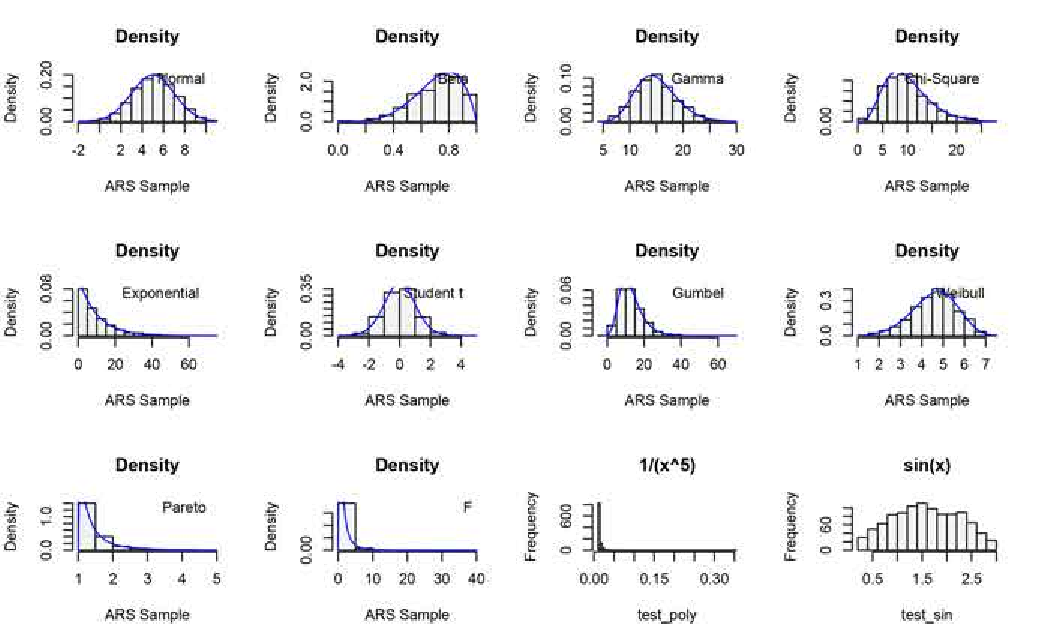
\includegraphics{12_Sampling_90per.pdf}


\section{Contributions of Members}
The group worked together through six face-to-face meetings.  At early stages of our work, we discussed the problem and all made contributions to our general approach and the pseudo-code of the algorithm for adaptive rejection sampling.  In later meetings, we all coded together and collaborated in areas that represented our individual strengths.  We made our work as cohesive as possible by asking questions and ensuring that all members were following the same line of analysis and coding style.

Chris wrote the core functions of the $\emph{ars()}$ function and developed the updating plotting method for the simulation.  He also pulled all of our final files into an R package.

Tom worked on the lower bound function, as well as vectorizing and debugging of $\emph{check.abscissae()}$ the (initial abscissae) function. Tom also wrote the test function for various known distributions and formatted the equations used in the paper in latex syntax.

Hairong helped work on the initial abscissae function (check.abscissae) used to create the starting $\emph{x}$ values for the ARS algorithm, and did preliminary work on the code for the sampling step.  She also wrote .Rd help files for half of the functions in our code.

Brittney helped work on the initialization ($\emph{check.abscissae()}$) function with Hairong, and wrote the other half of the .Rd help documentation.  Additionally, she drafted the written documentation to submit for the project.


Note: The project was submitted to bspace by Christian Carmona.



\end{document}
